\documentclass[a4paper,12pt]{article}
\usepackage[ngerman]{babel}
\usepackage{multirow}
\usepackage{xltxtra}
\usepackage[utf8x]{inputenc}
\usepackage{fontspec}
\usepackage{eurosym}
\usepackage{graphicx}
\usepackage[paper=a4paper,left=25mm,right=25mm,top=25mm,bottom=25mm]{geometry}
\usepackage{makecell}
\usepackage[table]{xcolor}
\usepackage[symbol]{footmisc}
\usepackage{float}
\usepackage[normalem]{ulem}
\usepackage{xcolor,colortbl}
\definecolor{Gray}{gray}{0.85}
\usepackage[automark]{scrlayer-scrpage}
\usepackage[
	colorlinks=true,
	urlcolor=blue,
	linkcolor=green
]{hyperref}
\setlength{\parindent}{0em}
\setlength{\parskip}{1ex}
\pagestyle{scrheadings}
\clearscrheadfoot
\usepackage[defaultsans]{droidsans}
\renewcommand*\familydefault{\sfdefault}
\begin{document}
\input{theme.tex}
\input{version.tex}
\newcommand{\combineDivisions}{Hinweis: Wenn weniger als 5 Teams in einer der
Altersgruppen angemeldet sind, hat die Veranstaltungsleitung die Möglichkeit,
Altersgruppen zusammenzulegen. }

\newcommand{\declareExhibition}{Wenn insgesamt weniger als 5 Teams angemeldet
sind kann die Veranstaltung zur Ausstellung erklärt werden. }

\newcommand{\robotRequirements}{Autonomer Roboter, basierend auf einer
beliebigen Plattform, der \euro{1.500} oder weniger kostet und die folgenden
Designbedingungen erfüllt, die beim Check-In überprüft werden:}


\newcommand{\tournamentScoring}{
\begin{figure}[H]
	\centering
	\def\svgwidth{\columnwidth}
	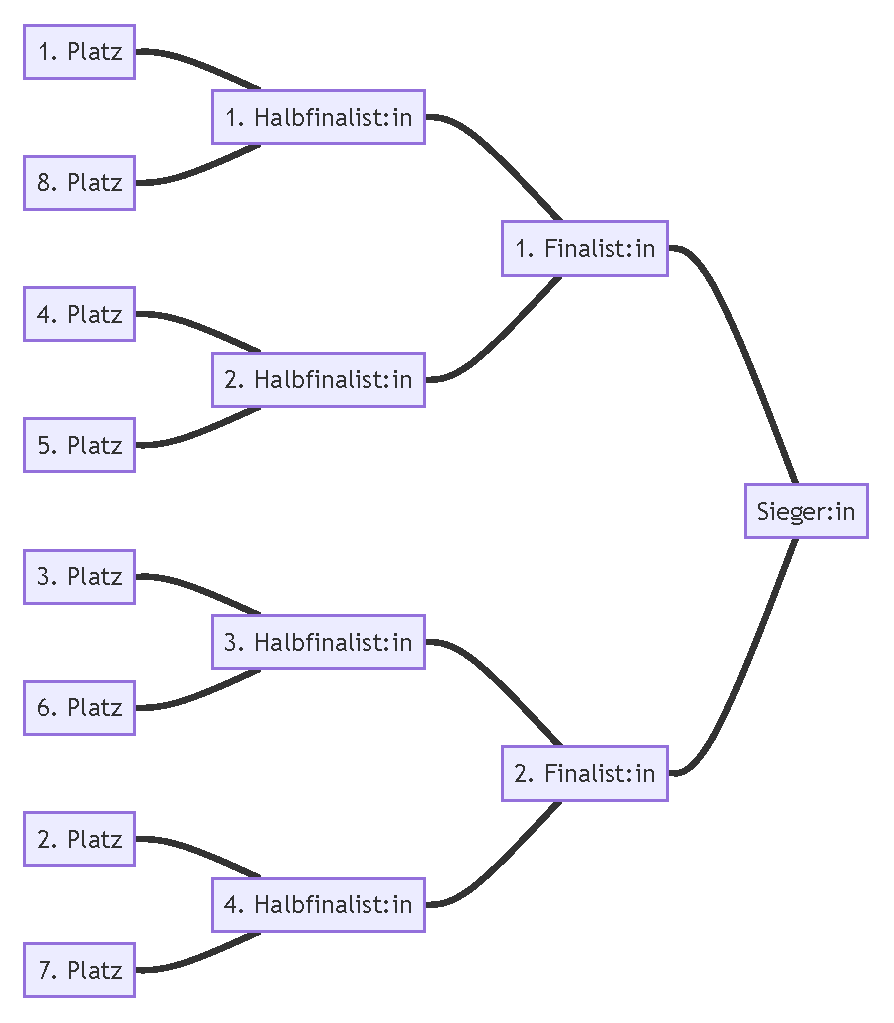
\includegraphics{tournament_score/tournament_score.pdf}
\end{figure}
}

\newcommand{\tournamentQualification}{Die aufsteigenden Teams werden
entsprechend ihrer Gesamtpunktzahl in den Turnierplan eingetragen (unten findet
ihr ein Beispiel für ein typisches Turnier mit 8 Teams). }

\newcommand{\combinedTournament}{
Hinweis: Wenn weniger als 8 Teams in allen Altersgruppen angemeldet sind, hat
die Veranstaltungsleitung die Möglichkeit, den Turnierplan entsprechend
anzupassen.
}

\newcommand{\scoreRuns}{
Die besten (8) Teams, welche am Turnier teilnehmen, werden wie folgt ermittelt:
\begin{itemize}
	\item Die Veranstaltungsleitung legt fest wieviele Läufe pro Team
		offiziell gewertet werden dürfen.
	\item Davon gehen die besten Wertungen in die Gesamtpunktzahl ein.
	\item Die Veranstaltungsleitung legt fest wieviele der offiziell
		gewerteten Läufen in die Gesamtpunktzahl eingehen.
	\item Auf Grundlage dieser Gesamtpunktzahl werden die besten Teams
		ermittelt, welche am Turnier teilnehmen.
\end{itemize}
}

\newcommand{\lightConditions}{
Die Challenge kann in Bereichen mit natürlichen Licht stattfinden, welches die
Lichtverhältnisse auf dem Spielplan verändern kann. Teams sollten darauf
vorbereitet sein, diese natürlichen Bedingungen zu meistern. }

\ohead{Regelstand: \commitDate, id: \commitID}
\title{\tagYear\ SUMO Challenge Regeln}

\makeatletter
\let\inserttitle\@title
\makeatother
\begin{center}
	\rrgerLogo
	\huge                      % Schriftgröße einstellen
	\bfseries                   % Fettdruck einschalten
	\\
	\inserttitle
\end{center}

\section{Ziel}
Entwerfe, baue und programmiere einen autonomen Roboter, der einen gegnerischen
Sumoroboter suchen und aus einem erhöhten Ring schieben kann.

\section{Altersgruppen/Masseklassen}
Bitte entnehme der untenstehenden Tabelle, in welcher Altersgruppe/Masseklasse
du antreten möchtest.
\begin{center}
	\begin{tabular}{|c|c|c|} \hline
		\multirow{2}*{1kg} & \multirow{2}*{3kg} \\
		& \\ \hline
		ES &  \\ \hline
		MS & \footnotemark[7]{} \\ \hline
		HS & HS \\ \hline
		\footnotemark[7] & UP \\ \hline
	\end{tabular}
	\footnotetext[7]{Diese Kategorien können nach Ermessen der
		Veranstaltungsleitung hinzugefügt werden.}
	\\ \vspace{\baselineskip}
\end{center}
\combineDivisions

\section{Anfoderungen}
\subsection{Roboter}
\robotRequirements
\begin{itemize}
	\item Die maximale Größe des Roboters beträgt 25 cm x 18 cm ohne
		Höhenbeschränkung, gemessen mit allen beweglichen Komponenten
		in ihrer Ausgangsposition.
	\item Größen- und Massenbeschränkungen werden während der gesamten
		Veranstaltung strikt durchgesetzt, um den Wettbewerb für alle
		Teilnehmer:innen fair zu gestalten.
	\item Bauteile mit Gelenken oder beweglichen Teilen sind zulässig,
		solange sie den oben genannten Konstruktionsregeln entsprechen.
		Es gilt jedoch die Regel "`kein vorsätzlicher Schaden"' - das
		bedeutet, dass Umwerfer (engl. "`flipper"' oder "`skid plate"')
		zwar in Ordnung sind, aber absichtlich zerstörende Mechanismen
		wie Schleifscheiben (engl. "`abrasive spinner"') oder Hämmer
		etc. nicht erlaubt sind.
\end{itemize}

\subsection{Wettbewerbsring}
Ein schwarzer (oder weißer) Kreis mit 100 cm Durchmesser und 5 cm weißem
(schwarzen) Rand auf einer 13 bis 20 mm dicken Platte. Die Oberfläche des Rings
sollte 50 bis 80 mm über dem Boden liegen. (die Maße können je nach den
verwendeten lokalen Materialien leicht variieren).
\\ \vspace{\baselineskip}

%TODO
%\includegraphics[width=1.0\textwidth]{images/sumo_bot_ring.png}

\section{Allgemeine Spielregeln und Wertung}
\begin{itemize}
	\item Jeder Roboter wird in einer Reihe von Rundenspielen antreten. Die
		Anzahl der Runden/Matches wird am Tag des Wettbewerb anhand der
		verfügbaren Zeit und der Anzahl von Robotern in jeder Kategorie
		festgelegt.
	\item Ein Spiel ist beendet, wenn ein Team zweimal gegen die
		Gegner:innen gewonnen hat. Für einen Sieg gibt es 3 Punkte, für
		ein Unentschieden 1 Punkt und für eine Niederlage 0 Punkte.
	\item Die Punkte der Teams werden während des Wettkampfs gezählt und
		angezeigt. Die besten 8 Teams in jeder Kategorie werden für die
		Endspiele ausgewählt.
	\item Die Teams können auf freien Spielfeldern üben, wobei sie sich mit
		anderen übenden Teams abwechseln müssen.
	\item Die Roboter beginnen, indem sie die weiße (schwarze) Linie an den
		einander gegenüberliegenden Seiten des Tisches berühren. Sie
		können in jeder beliebigen Ausrichtung positioniert werden. Die
		Roboter müssen nach dem Drücken der Starttasten 3 Sekunden lang
		pausieren, damit sich das Teammitglied vom Ring entfernen kann.
	\item Verloren hat der Roboter, der den Ring zuerst verlässt, d.h. die
		Oberfläche berührt, auf der der Wettbewerbsring platziert ist.
		Der Punktrichter kann nach eigenem Ermessen nach 60 Sekunden
		ein Unentschieden verkünden oder bei "`gesperrten Robotern"'
		nach 5 Sekunden einen Neustart anordnen.
	\item Die Bediener:innen des Roboters dürfen diesen nur auf Anweisung
		der Punktrichter:innen berühren. Für jedes Spiel sind 5 Minuten
		vorgesehen. Wenn es in dieser Zeit keinen Sieg gibt, wird es
		als unentschieden gewertet.
	\item Konfliktlösung - während des Spiels sind die Entscheidungen der
		Punktrichter:innen endgültig.
\end{itemize}

\pagebreak
\section{Turnierplan}
\begin{itemize}
	\item In der Regel richten wir Turniere für die besten 8 Teams aus.
		Sollte es jedoch aufgrund von Unentschieden mehr als 8 Teams
		geben, kann die Veranstaltungsleitung die Turniergröße auf 12
		oder 16 Teams erhöhen oder ein Tie-Breaker-Turnier
		veranstalten, um auf 8, 12 oder 16 Teams zu kommen, um ein
		Turnier auszurichten.
        \item \tournamentQualification
\end{itemize}
\tournamentScoring
\end{document}
